
\section{重修线性代数2——具象}
抽象数学概念的直观想象,是从最基本的概念开始,用已经习惯的具象,层层堆积建造而成。物理是描述现实的世界,其中的概念都经事例反复喻解,而能直观想象,任何认知的偏差,都以事实为依据来纠正。数学研究逻辑建构的抽象世界,在那里公理和定义是最终的依据,定理是可信的构件。数学为了强调逻辑推理是求证的唯一手段,防止学生误用事实和想象作依据,多数课文故意剥离抽象概念来源的事例来避免过度想象,一切通过定义和逻辑证明。这样的数学训练严谨了,学生却往往失去了有用的直观。对于数学概念和定理,直观想象因人而异使用的边际不同,都不足为凭求真,只有逻辑证明才是可靠的,但有了它能将缤纷的美色编织成图案,会指引你在这抽象世界里行走。正确的想象是由基础概念和定理累积而成的,它必须在自己头脑中通过逻辑证明的反复纠偏淬炼才有价值。

这篇用列向量和矩阵的具象,让读者回顾学过线性代数的基本概念,建立起基本图像。这里常对一个概念从不同角度做不同的解读,用心的读者可从不同的方向看到图像的不同侧面。这些都是非常基本的,大多是你已经熟悉的,但也可能有你过去忽略的视角。
\subsection{列向量和矩阵}
解析几何告诉我们,几何空间中一个点可以用它的坐标,也就是用一组数来表示。这组数也表示,从原点到这点的矢量分解在各坐标轴方向上的分量。用几何的语言来说,坐标值即是向量在坐标轴上投影的长度;向量是坐标轴单位向量的线性组合,这线性组合的系数是这些投影分量的长度;包含着这些向量的几何空间叫做向量空间。竖排着坐标值的一组数,称为列向量,或统称为向量;数组中每个数称为它的分量。

\begin{figure}[h]
	\centering
	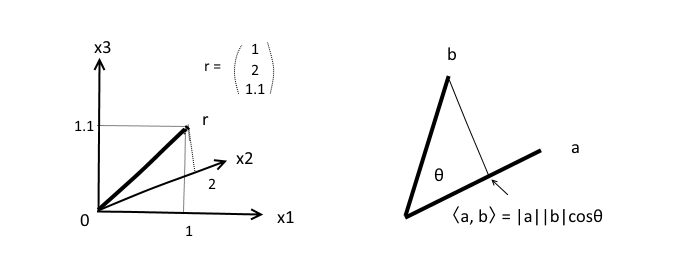
\includegraphics[width=0.7\linewidth]{pic/153404gr2s818g3sg3g1h9.png}
	\caption{向量示意图}
	\label{fig:153404gr2s818g3sg3g1h9}
\end{figure}


列向量相加等于对应的分量相加;数乘等于它乘以向量的每个分量。用$ n $个实数表示列向量的线性空间通常记为$ R^n $,其内积等于两个向量对应分量乘积后的总和,它是向量投影与投向向量长度的乘积。

用一个数组的列向量表示$ n $维线性空间中向量,以此类比三维物理空间的矢量,从三维的物理空间来推想多维的线性空间;用列向量的内积计算向量对另一个向量方向的投影长度,想象向量方向间的夹角;矩阵乘列向量,得到另一个列向量,这表示了线性算子的映射作用,不难用计算来验证这个映射是线性的。

\subsection{矩阵运算}
列向量和矩阵是线性代数中抽象概念的具体表达和运算手段。列向量可以看成仅有一列的矩阵,它的运算规则可以归纳在矩阵中来介绍。

矩阵是排列成矩形的一组数,$ m*n $矩阵是m行n列的矩阵,$ m*n $矩阵$ A=(a_{ij})_{mn} $和$ B=(b_{ij})_{mn} $相加是矩阵中相同位置的各元素相加,$ A+B=(a_{ij}+b_{ij})_{mn} $;数乘c则是c乘以矩阵A中的每一个元素$ c*A=(c*a_{ij})_{mn} $.

显然,$ m*n $矩阵相加及与数相乘仍然是$ m*n $矩阵,这叫做对线性运算封闭,即$ m*n $矩阵构成了一个线性空间。一行数组是$ 1*n $的矩阵,称为行向量;一列数组是$ m*1 $的矩阵,称为列向量,它们分别也构成了线性空间。虽然矩阵也构成线性空间,一般我们都把线性空间的元素表示成向量的形式,而用矩阵表示线性空间中的线性算子。这是在向量和算子的坐标表示中,形成的约定。

$ m*n $矩阵$ A $与$ n*k $矩阵$ D $相乘$ AD $是一个$ m*k $的矩阵$ G=AD $,其中$ G $第$ i $行第$ j $列元素定义为$ A $中第$ i $行与$ D $中第$ j $列的内积,$ G=(g_{ij})_{mk} $, $ g_{ij}= \sum_{k}^{r}a_{ir}b_{rj} $ 。

任意的矩阵相乘未必都有定义,相乘的矩阵,左边矩阵的列数必须等于右边矩阵的行数。在有定义的矩阵乘法中,显然乘法的交换律是不成立的,但多个矩阵相乘,结合律是成立的。矩阵与向量的相乘可以看作矩阵相乘的特殊情况。

乘法的交换律不成立,这在矩阵乘法算法定义下导出,也许人们不觉为奇,但是把矩阵看成是一个数学的实体,看成是线性算子的数值表示,用一个字母符号代表它,解读成一个物理变量,相乘交换律不成立,就与长期直观形成标量的代数运算相冲突。这是矩阵给经验数学之人第一个深刻的习惯改变。如果你不经意,错误的习惯会在以后继续迷惑你。量子力学奠基人之一海森堡创立矩阵力学时,曾为此苦恼过,物理学者当时难以接受也因不习惯于此。

抽象代数运算,原则上可以定义不同的矩阵乘法,例如在$ m*n $矩阵间定义同下标的元素相乘,实际上这种乘法在支持矩阵计算的软件中,叫做元素运算(Element-Wise Operations),非常有用。但是通常的矩阵乘列向量的算法定义,来自线性方程组中算子对向量作用的表达,约定的矩阵乘法定义来自复合算子的表达,这个约定乘法的设计,构建了线性代数的大厦。

\subsection{基本图像}
历史中,矩阵来自解线性方程组。往下看个具体的例子。
\begin{gather*}
	x_1+x_2=3\\
	x_1+x_2+2x_3=9\\
	x_1+2x_2+2x_3=11
\end{gather*}

这是一个线性方程组。将方程左边的系数,未知数和方程右边的数,由矩阵乘法的定义,可以写成矩阵的形式,则是:
%    \[ \begin{pmatrix} a&b\\c&d \end{pmatrix} \quad
%\begin{bmatrix} a&b\\c&d \end{bmatrix} \quad
%\begin{Bmatrix} a&b\\c&d \end{Bmatrix} \quad
%\begin{vmatrix} a&b\\c&d \end{vmatrix} \quad
%\begin{Vmatrix} a&b\\c&d \end{Vmatrix} \]

\begin{gather*}
	\begin{pmatrix} 1&1&0\\1&1&2\\1&2&2 \end{pmatrix} \begin{pmatrix} x_1\\x_2\\x_3 \end{pmatrix}=
	\begin{pmatrix}	3\\9\\11 \end{pmatrix}
\end{gather*}

分别用$ A $, \textbf{x}, \textbf{b}, 记这三个矩阵。方程用这些符号可以表示如下:

\begin{gather*}
A = \begin{pmatrix} 1&1&0\\1&1&2\\1&2&2 \end{pmatrix}, x = \begin{pmatrix} x_1\\x_2\\x_3 \end{pmatrix},b = 	\begin{pmatrix}	3\\9\\11 \end{pmatrix}, \mathbf{ Ax = b }
\end{gather*}

列向量这一组数表示线性空间中一个向量,方程式子$ \bm{ Ax=b } $ 表示矩阵$ \bm{A}$将向量$ \bm{x}$变成向量$ \bm{b}$。矩阵$ \bm{A}$的作用如同函数,实现一个映射,在空间中称为算子。这是方程、矩阵和空间中向量间最基本的关系。

矩阵乘列向量,是矩阵作为一个线性算子把这列向量映射成另一个列向量,线性方程组用计算的细节反映了这种关系。注意方程的个数未必要等于未知数的个数,即它表示成的矩阵不一定是方阵。这个方程右边的向量未必在映射算子的值域中,即解未必存在。即使它在值域中,也许它不只是一个映射的像,即解即使存在也未必是唯一的。你要从中学习惯的特殊情况中走出来。

从另一个角度,线性方程组的每一行对应着一个行向量与向量$ \bm{x} $的内积计算,方程的右边是内积的值。它表示着向量间的投影关系。

\begin{gather*}
	B_1 = \begin{pmatrix}
		1\\1\\0
	\end{pmatrix},
	B_2 = \begin{pmatrix}
		1\\1\\2
	\end{pmatrix},
	B_3 = \begin{pmatrix}
		1\\2\\2
	\end{pmatrix} \quad
	A = \begin{pmatrix}
		B_1^T\\B_2^T\\B_3^T
	\end{pmatrix},
	\begin{matrix}
		<B_1,\bm{x}>=3\\
		<B_2,\bm{x}>=9\\
		<B_3,\bm{x}>=11
	\end{matrix}
\end{gather*}

两个矩阵相乘既可以看成两个线性算子的复合,也可以看成用右边矩阵的列向量为线性组合的系数,在左边矩阵的列向量上构造出了一组的列向量,形成的另一个矩阵。

矩阵是数据的一种形式表示,其加法和乘法对应着它们元素间按它的规则运算。矩阵中的元素通常是一个数,但不限于此,它可以是任何数学实体,如矩阵、算符等,只要相应的元素间运算有意义。我们可以把矩阵分块表示和运算,这有时可以带来运算方便和解释意义。例如上面的方程可以用分块矩阵形式表示为:

\begin{gather*}
	\begin{pmatrix}
		A_1&A_2&A_3
	\end{pmatrix}
	\begin{pmatrix}
		x_1\\x_2\\x_3
	\end{pmatrix}=
	\begin{pmatrix}
		3\\9\\11
	\end{pmatrix}
	\mbox{其中} \ 
	A_1 = \begin{pmatrix}
		1\\1\\1
	\end{pmatrix},
	A_2 = \begin{pmatrix}
		1\\1\\2
	\end{pmatrix},
	A_3 = \begin{pmatrix}
		0\\2\\2
	\end{pmatrix}
\end{gather*}

它表示方程右边的向量是向量$ A_1,A_2,A_3 $的线性组合,$ x $是这线性组合系数的那组数。把矩阵看成是排成一行的一组列向量,它乘右边的列向量,相当于用右边列向量的那组数把矩阵中的列向量线性组合成一个向量。解线性方程组可以看成求这个线性组合的系数。

\begin{gather*}
	x_1 \begin{pmatrix}
		1\\1\\1
	\end{pmatrix}+
	x_2 \begin{pmatrix}
		1\\1\\2
	\end{pmatrix}+
	x_3 \begin{pmatrix}
		0\\2\\2
	\end{pmatrix}=
	\begin{pmatrix}
		3\\9\\11
	\end{pmatrix}		
\end{gather*}

\subsection{计算工具}
从计算的角度,矩阵是排列成矩形的一组数,它们打包起来用一个数学符号代表以便于批量计算和引用。其加法和数乘来自向量空间的线性,而乘法的定义则为了适用于线性组合的表示。

矩阵在计算机里是个数组,可以用这个数据结构,储存诸如一张图片的像素,一个代数方程的系数,一个季度销售的列表和实验的数据等等,在计算机语言中用一个变量来表示。它们间的运算,除了矩阵的加减乘除指数运算外,还可以定义分别对应于每个元素间的运算,例如两矩阵的元素乘法和矩阵的初等函数计算。

矩阵的计算和图像显示在今日,已经是非常基本的科研和工程的工具了。我们学习线性代数必须明白矩阵各种计算的含义和算法,通过笔算的练习掌握它。但实际工作中,如果还停留于手算,就像仍然停留在手工作业不能融入工业时代一样的落后。

在21世纪,人机互动将成为最有效率的工作方式。过去直接引用数学定理来做科研,现在直接使用计算机中的软件来协助。矩阵和图像是一种非常通用的数据表达方式,已经有许多的计算机软件提供人机互动的界面和解释程序为此工作。用于数学、统计、科学和工程中,基于矩阵计算最有名的软件是MATLAB,这是个收费商业软件。在你的手头,如果没买这个软件,建议装一个GNU免费软件Octave,它的解释程序语言与MATLAB几乎一样,而且功能非常相似。在你的学习中可以用它验证计算,熟悉它用于工作。你可在GNU官网链接中下载这个免费软件

https://www.gnu.org/software/octave/

下面是在Octave(MATLAB也一样)指令窗中,演示上述例子的线性方程组解的计算,以及用两个和三个行向量分别表示二维和三维曲线100个点的坐标来画图。用户在“$ >> $”字符开始的行,打进指令,在那行下面,指令窗口直接打印出结果,如果在指令的末尾加上分号“;”,则不打印出结果,指令行中“\%”后面是解释文字。没有用过这软件的读者,建议花几个种头读一篇入门介绍的例子,如Introductionto Octave练习一遍。熟悉这类软件的使用,就像过去学了数学有关的计算,要熟悉对数表,计算尺,计算器使用一样的重要了。
\begin{table}[htbp]
	\setlength{\abovecaptionskip}{0.cm}%%%%这个还不大清楚意思
	%\caption{Nomenclature}
	%\label{Nomenclature}
	\centering
	\setlength{\tabcolsep}{2pt}
	
\begin{tabular}{|p{170 pt}|p{170 pt}|}

	\hline
	$ >> $ A = [1 1 0;  1 1 2; 1 2 2] \%矩阵
	
	A =
	
	1    1   0
	
	1    1   2
	
	1    2   2
	
	$ >> $ b = [3;  9; 11]  \%赋值列向量 b
	
	b =
	
	3
	
	9
	
	11
	
	$ >> $ x = Ab  \%用A左除法解 Ax=b 方程
	
	x =
	
	1
	
	2
	
	3
	
	$ >> $ A*x  %验证x是方程的解
	
	ans =
	
	3
	
	9
	
	11
	
	&
	
	t 是从0到5π有100个元素的行向量
	
	$ >> $t =  linspace(0, 5*pi, 100);  
	
	$ >> $plot(t,sin(t));                   
	
	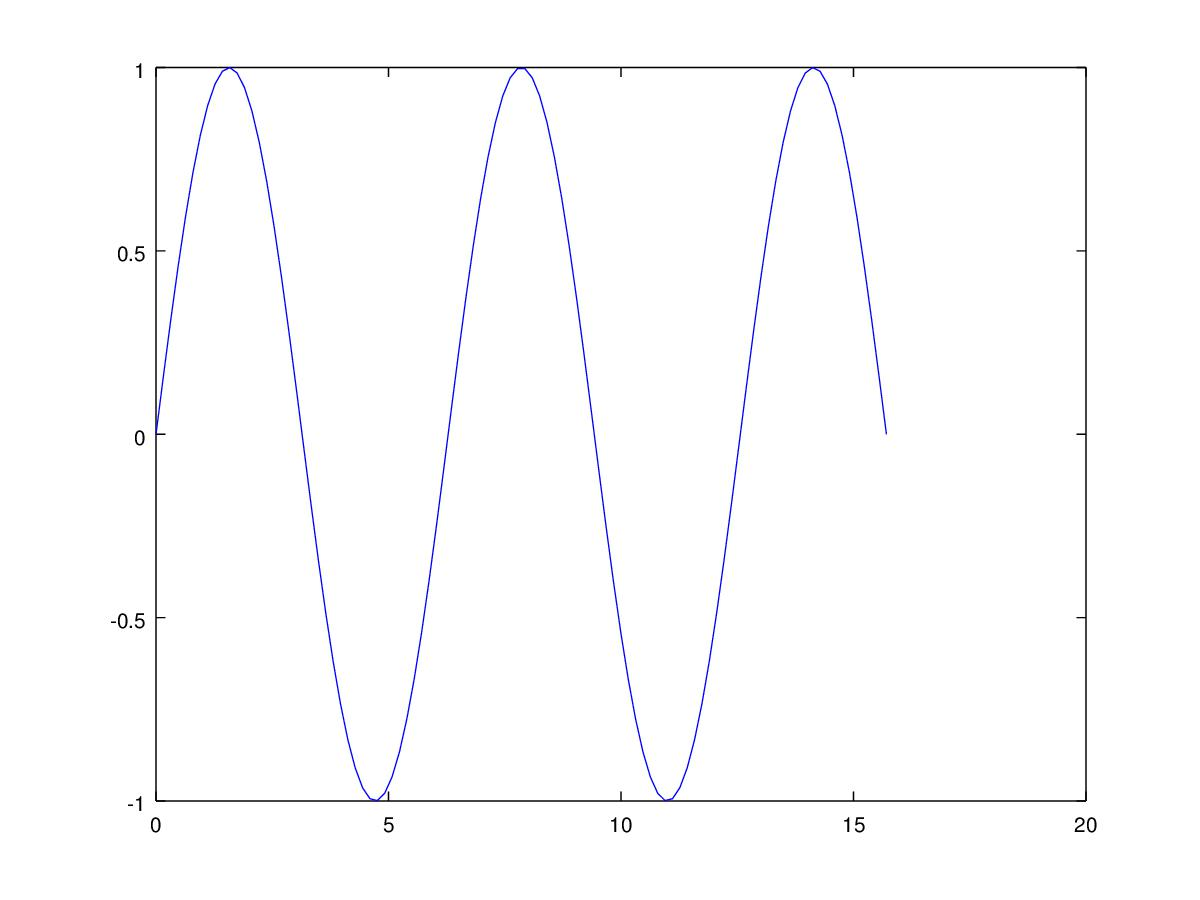
\includegraphics[width = .4\textwidth]{pic/154012hzzaaow33s7a7kst.jpg}
	
	$ >> $plot3(sin(t),cos(t),t);
	
	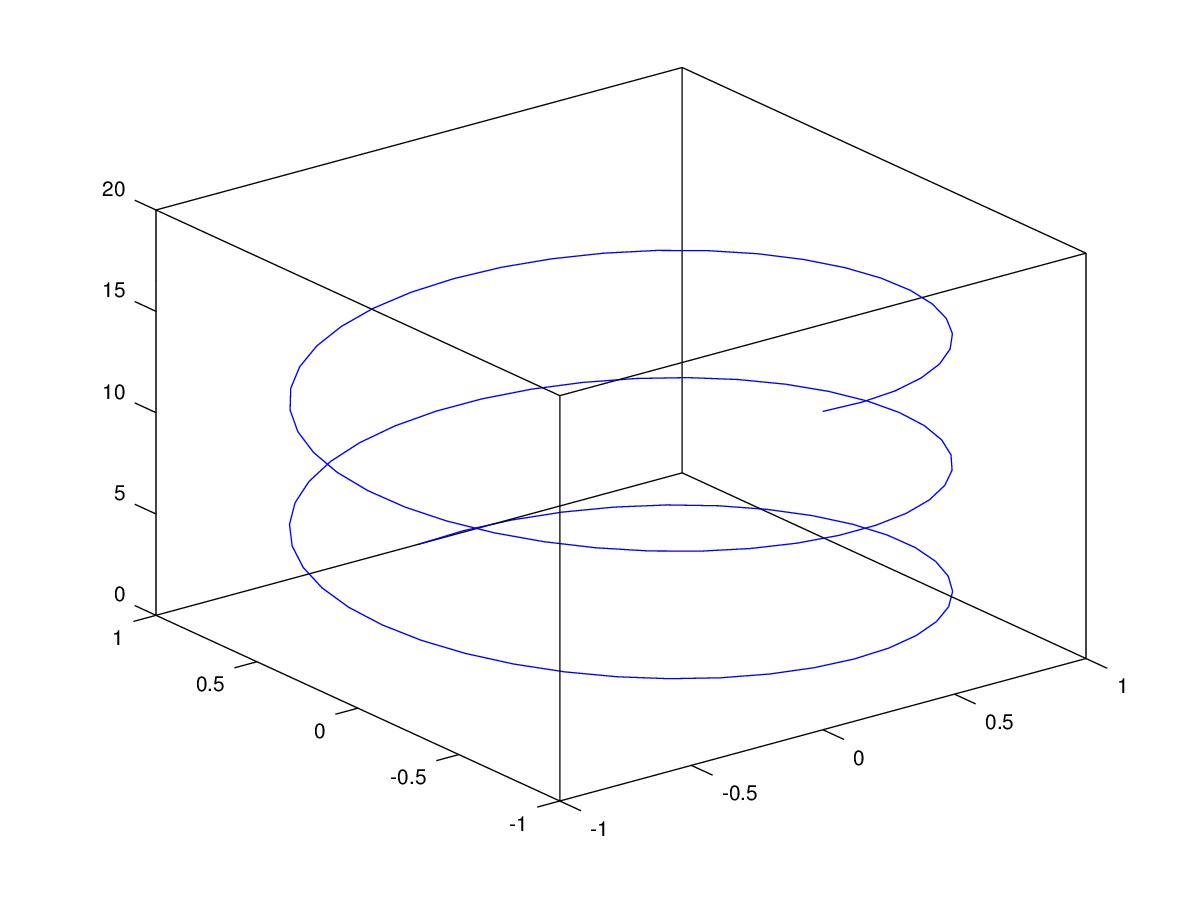
\includegraphics[width = .4\textwidth]{pic/154013uf11jfijj1nivsjn.jpg}\\
	\hline
\end{tabular}

\vspace{1.5em}%%%%%%%%%%%%%%%%%%%%缩减竖直距离%%%%%%%%%%%%%%%%%%%%%%
\end{table}
在这例子画出三维图后,用户还能用鼠标在图上旋转不同角度来观察这个空间曲线。这几个极其简单的例子,目的是给读者一个印象,用计算机可以很方便地进行矩阵计算和画图。它也是现代课程学习常用的工具。如果你还没用过,不妨现在开始熟悉它。
